\documentclass[border=0pt]{standalone}
\usepackage{iftex}
\ifPDFTeX
  \usepackage[T1]{fontenc}
  \usepackage{DejaVuSans}
  \renewcommand*\familydefault{\sfdefault}
  \usepackage[italic]{mathastext}
\else
  \usepackage{unicode-math}
  \setmainfont{DejaVuSans.ttf}[BoldFont=DejaVuSans-Bold.ttf,ItalicFont=DejaVuSans-Oblique.ttf,
    BoldItalicFont=DejaVuSans-BoldOblique.ttf]
  \setmathfont{texgyredejavu-math.otf}
\fi
\ifPDFTeX  % one glyph of matplotlib mathtext, by Unicode code point (hex)
  \def\mplchar#1{\ifnum"#1="2212 \ensuremath{-}\else\ifnum"#1="D7 \texttimes\else\char"#1\relax\fi\fi}
\else
  \def\mplchar#1{\char"#1\relax}
\fi
\frenchspacing  % matplotlib puts a normal space after punctuation
\usepackage{pgfplots}
\pgfplotsset{compat=1.18}
% matplotlib marker shapes; \pgfplotmarksize = half the matplotlib marker size
\pgfdeclareplotmark{mpl-o}{\pgfpathcircle{\pgfpointorigin}{\pgfplotmarksize}\pgfusepathqfillstroke}
\pgfdeclareplotmark{mpl-o-open}{\pgfpathcircle{\pgfpointorigin}{\pgfplotmarksize}\pgfusepathqstroke}
\pgfdeclareplotmark{mpl-s}{\pgfpathrectangle{\pgfpoint{-\pgfplotmarksize}{-\pgfplotmarksize}}{\pgfpoint{2\pgfplotmarksize}{2\pgfplotmarksize}}\pgfusepathqfillstroke}
\pgfdeclareplotmark{mpl-s-open}{\pgfpathrectangle{\pgfpoint{-\pgfplotmarksize}{-\pgfplotmarksize}}{\pgfpoint{2\pgfplotmarksize}{2\pgfplotmarksize}}\pgfusepathqstroke}
\def\mpltriangle#1{\pgfpathmoveto{\pgfpoint{0pt}{#1\pgfplotmarksize}}\pgfpathlineto{\pgfpoint{-\pgfplotmarksize}{-#1\pgfplotmarksize}}\pgfpathlineto{\pgfpoint{\pgfplotmarksize}{-#1\pgfplotmarksize}}\pgfpathclose}
\pgfdeclareplotmark{mpl-^}{\mpltriangle{}\pgfusepathqfillstroke}
\pgfdeclareplotmark{mpl-^-open}{\mpltriangle{}\pgfusepathqstroke}
\pgfdeclareplotmark{mpl-v}{\mpltriangle{-}\pgfusepathqfillstroke}
\pgfdeclareplotmark{mpl-v-open}{\mpltriangle{-}\pgfusepathqstroke}
\def\mpldiamond{\pgfpathmoveto{\pgfpoint{0pt}{1.41421\pgfplotmarksize}}\pgfpathlineto{\pgfpoint{-1.41421\pgfplotmarksize}{0pt}}\pgfpathlineto{\pgfpoint{0pt}{-1.41421\pgfplotmarksize}}\pgfpathlineto{\pgfpoint{1.41421\pgfplotmarksize}{0pt}}\pgfpathclose}
\pgfdeclareplotmark{mpl-D}{\mpldiamond\pgfusepathqfillstroke}
\pgfdeclareplotmark{mpl-D-open}{\mpldiamond\pgfusepathqstroke}
\pgfdeclareplotmark{mpl-x}{\pgfpathmoveto{\pgfpoint{-\pgfplotmarksize}{-\pgfplotmarksize}}\pgfpathlineto{\pgfpoint{\pgfplotmarksize}{\pgfplotmarksize}}\pgfpathmoveto{\pgfpoint{-\pgfplotmarksize}{\pgfplotmarksize}}\pgfpathlineto{\pgfpoint{\pgfplotmarksize}{-\pgfplotmarksize}}\pgfsetbuttcap\pgfusepathqstroke}
\pgfdeclareplotmark{mpl-+}{\pgfpathmoveto{\pgfpoint{-\pgfplotmarksize}{0pt}}\pgfpathlineto{\pgfpoint{\pgfplotmarksize}{0pt}}\pgfpathmoveto{\pgfpoint{0pt}{-\pgfplotmarksize}}\pgfpathlineto{\pgfpoint{0pt}{\pgfplotmarksize}}\pgfsetbuttcap\pgfusepathqstroke}
\def\mplplus{\pgfpathmoveto{\pgfpoint{-0.33333\pgfplotmarksize}{-\pgfplotmarksize}}\pgfpathlineto{\pgfpoint{0.33333\pgfplotmarksize}{-\pgfplotmarksize}}\pgfpathlineto{\pgfpoint{0.33333\pgfplotmarksize}{-0.33333\pgfplotmarksize}}\pgfpathlineto{\pgfpoint{\pgfplotmarksize}{-0.33333\pgfplotmarksize}}\pgfpathlineto{\pgfpoint{\pgfplotmarksize}{0.33333\pgfplotmarksize}}\pgfpathlineto{\pgfpoint{0.33333\pgfplotmarksize}{0.33333\pgfplotmarksize}}\pgfpathlineto{\pgfpoint{0.33333\pgfplotmarksize}{\pgfplotmarksize}}\pgfpathlineto{\pgfpoint{-0.33333\pgfplotmarksize}{\pgfplotmarksize}}\pgfpathlineto{\pgfpoint{-0.33333\pgfplotmarksize}{0.33333\pgfplotmarksize}}\pgfpathlineto{\pgfpoint{-\pgfplotmarksize}{0.33333\pgfplotmarksize}}\pgfpathlineto{\pgfpoint{-\pgfplotmarksize}{-0.33333\pgfplotmarksize}}\pgfpathlineto{\pgfpoint{-0.33333\pgfplotmarksize}{-0.33333\pgfplotmarksize}}\pgfpathclose}
\pgfdeclareplotmark{mpl-P}{\mplplus\pgfusepathqfillstroke}
\pgfdeclareplotmark{mpl-P-open}{\mplplus\pgfusepathqstroke}
\def\mplstar{\pgfpathmoveto{\pgfpointpolar{90}{\pgfplotmarksize}}%
  \foreach \i in {1,...,4} {\pgfpathlineto{\pgfpointpolar{90+72*\i-36}{0.381966\pgfplotmarksize}}\pgfpathlineto{\pgfpointpolar{90+72*\i}{\pgfplotmarksize}}}%
  \pgfpathlineto{\pgfpointpolar{54}{0.381966\pgfplotmarksize}}\pgfpathclose}
\pgfdeclareplotmark{mpl-*}{\mplstar\pgfusepathqfillstroke}
\pgfdeclareplotmark{mpl-*-open}{\mplstar\pgfusepathqstroke}
\def\mpltriside#1{\pgfpathmoveto{\pgfpoint{#1\pgfplotmarksize}{0pt}}\pgfpathlineto{\pgfpoint{-#1\pgfplotmarksize}{\pgfplotmarksize}}\pgfpathlineto{\pgfpoint{-#1\pgfplotmarksize}{-\pgfplotmarksize}}\pgfpathclose}
\pgfdeclareplotmark{mpl-<}{\mpltriside{-}\pgfusepathqfillstroke}
\pgfdeclareplotmark{mpl-<-open}{\mpltriside{-}\pgfusepathqstroke}
\pgfdeclareplotmark{mpl->}{\mpltriside{}\pgfusepathqfillstroke}
\pgfdeclareplotmark{mpl->-open}{\mpltriside{}\pgfusepathqstroke}
\def\mplpolygon#1{\pgfpathmoveto{\pgfpointpolar{90}{\pgfplotmarksize}}\foreach \i in {1,...,#1} {\pgfpathlineto{\pgfpointpolar{90+360/#1*\i}{\pgfplotmarksize}}}\pgfpathclose}
\pgfdeclareplotmark{mpl-p}{\mplpolygon{5}\pgfusepathqfillstroke}
\pgfdeclareplotmark{mpl-p-open}{\mplpolygon{5}\pgfusepathqstroke}
\pgfdeclareplotmark{mpl-h}{\mplpolygon{6}\pgfusepathqfillstroke}
\pgfdeclareplotmark{mpl-h-open}{\mplpolygon{6}\pgfusepathqstroke}
\definecolor{mplc0}{HTML}{B0B0B0}
\definecolor{mplc1}{HTML}{000000}
\definecolor{mplc2}{HTML}{DAA520}
\begin{document}
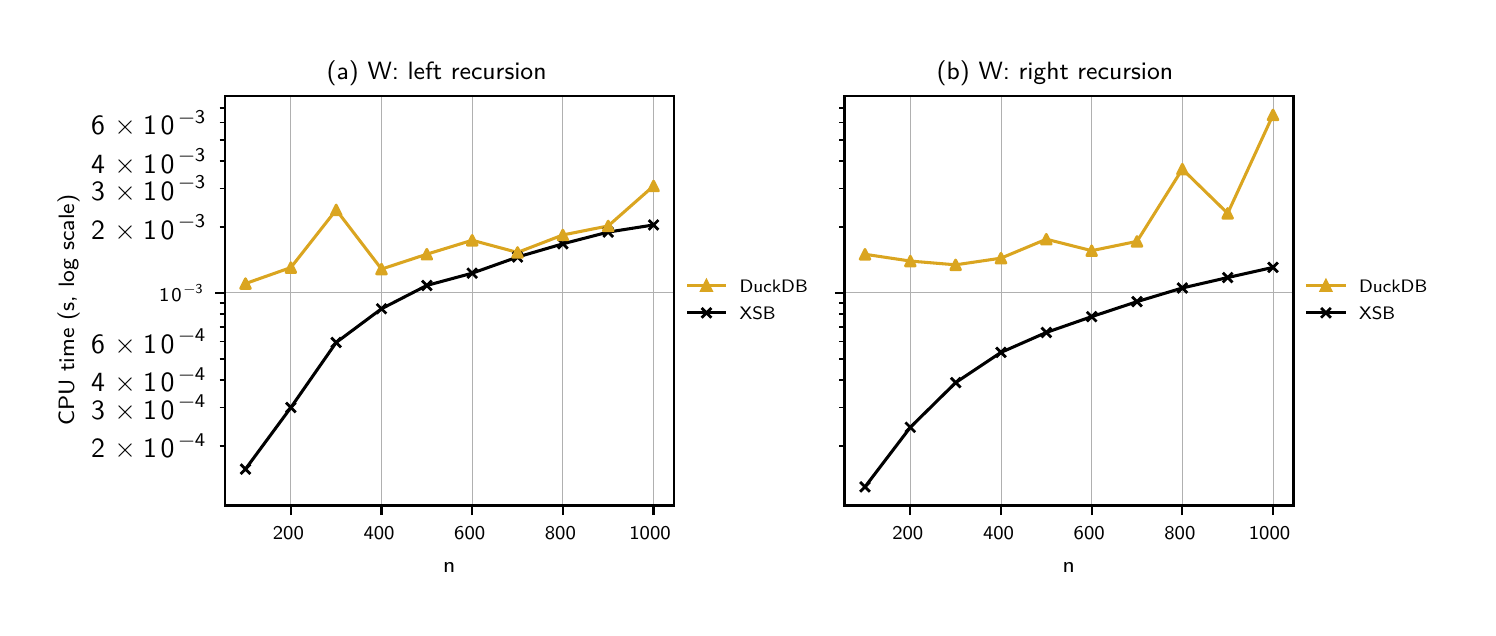
\begin{tikzpicture}
\useasboundingbox (0in,0in) rectangle (7.2in,2.9in);
\begin{axis}[at={(0.9872in,0.5111in)}, anchor=south west, scale only axis, width=2.2443in, height=2.0456in, xmin=55, xmax=1045, ymin=0.0001069040563, ymax=0.007904527008, enlargelimits=false, clip=true, axis on top=false, axis line style={line width=0.8bp, black}, tick align=outside, tick pos=left, major tick length=3.5bp, minor tick length=2bp, major tick style={line width=0.8bp, black}, minor tick style={line width=0.6bp, black}, xticklabels={}, yticklabels={}, scaled x ticks=false, scaled y ticks=false, xlabel={}, ylabel={}, title={}, xtick={200,400,600,800,1000}, minor xtick={}, ymode=log, log basis y=10, ytick={0.001}, minor ytick={0.0002,0.0003,0.0004,0.0005,0.0006,0.0007,0.0008,0.0009,0.002,0.003,0.004,0.005,0.006,0.007}, xmajorgrids, ymajorgrids, major grid style={line width=0.3bp, draw=mplc0}]
\addplot[color=mplc1, line width=1.1bp, line join=round, solid, line cap=rect, mark=mpl-x, mark size=1.75bp, mark options={solid, line width=1bp, draw=mplc1}] coordinates {(100,0.0001568) (200,0.0002994) (300,0.0005936) (400,0.0008464) (500,0.0010816) (600,0.0012302) (700,0.0014578) (800,0.0016756) (900,0.001896) (1000,0.0020434)};
\addplot[color=mplc2, line width=1.1bp, line join=round, solid, line cap=rect, mark=mpl-^, mark size=1.75bp, mark options={solid, line width=1bp, draw=mplc2, fill=mplc2}] coordinates {(100,0.0011032) (200,0.0013052) (300,0.0023948) (400,0.0012844) (500,0.0015024) (600,0.0017394) (700,0.0015304) (800,0.0018392) (900,0.0020224) (1000,0.0030784)};
\end{axis}
\begin{axis}[at={(4.0846in,0.5111in)}, anchor=south west, scale only axis, width=2.2443in, height=2.0456in, xmin=55, xmax=1045, ymin=0.0001069040563, ymax=0.007904527008, enlargelimits=false, clip=true, axis on top=false, axis line style={line width=0.8bp, black}, tick align=outside, tick pos=left, major tick length=3.5bp, minor tick length=2bp, major tick style={line width=0.8bp, black}, minor tick style={line width=0.6bp, black}, xticklabels={}, yticklabels={}, scaled x ticks=false, scaled y ticks=false, xlabel={}, ylabel={}, title={}, xtick={200,400,600,800,1000}, minor xtick={}, ymode=log, log basis y=10, ytick={0.001}, minor ytick={0.0002,0.0003,0.0004,0.0005,0.0006,0.0007,0.0008,0.0009,0.002,0.003,0.004,0.005,0.006,0.007}, xmajorgrids, ymajorgrids, major grid style={line width=0.3bp, draw=mplc0}]
\addplot[color=mplc1, line width=1.1bp, line join=round, solid, line cap=rect, mark=mpl-x, mark size=1.75bp, mark options={solid, line width=1bp, draw=mplc1}] coordinates {(100,0.00013) (200,0.0002432) (300,0.0003892) (400,0.0005348) (500,0.0006596) (600,0.000779) (700,0.000912) (800,0.0010528) (900,0.001175) (1000,0.0013074)};
\addplot[color=mplc2, line width=1.1bp, line join=round, solid, line cap=rect, mark=mpl-^, mark size=1.75bp, mark options={solid, line width=1bp, draw=mplc2, fill=mplc2}] coordinates {(100,0.001501) (200,0.0013976) (300,0.0013432) (400,0.001441) (500,0.001759) (600,0.001559) (700,0.001719) (800,0.0036762) (900,0.0023082) (1000,0.0065002)};
\end{axis}
\draw[color=mplc2, line width=1.1bp, line join=round, solid, line cap=rect] (3.3038in,1.6097in) -- (3.4843in,1.6097in);
\begin{scope}[solid, line width=1bp, draw=mplc2, fill=mplc2]\pgftransformshift{\pgfpoint{3.394in}{1.6097in}}\pgfsetplotmarksize{1.75bp}\pgfuseplotmark{mpl-^}\end{scope}
\draw[color=mplc1, line width=1.1bp, line join=round, solid, line cap=rect] (3.3038in,1.4743in) -- (3.4843in,1.4743in);
\begin{scope}[solid, line width=1bp, draw=mplc1]\pgftransformshift{\pgfpoint{3.394in}{1.4743in}}\pgfsetplotmarksize{1.75bp}\pgfuseplotmark{mpl-x}\end{scope}
\draw[color=mplc2, line width=1.1bp, line join=round, solid, line cap=rect] (6.4011in,1.6097in) -- (6.5817in,1.6097in);
\begin{scope}[solid, line width=1bp, draw=mplc2, fill=mplc2]\pgftransformshift{\pgfpoint{6.4914in}{1.6097in}}\pgfsetplotmarksize{1.75bp}\pgfuseplotmark{mpl-^}\end{scope}
\draw[color=mplc1, line width=1.1bp, line join=round, solid, line cap=rect] (6.4011in,1.4743in) -- (6.5817in,1.4743in);
\begin{scope}[solid, line width=1bp, draw=mplc1]\pgftransformshift{\pgfpoint{6.4914in}{1.4743in}}\pgfsetplotmarksize{1.75bp}\pgfuseplotmark{mpl-x}\end{scope}
\node[anchor=base west, inner sep=0pt, text=mplc1, font=\fontsize{7bp}{8.4bp}\selectfont] at (1.2232in,0.34in) {200};
\node[anchor=base west, inner sep=0pt, text=mplc1, font=\fontsize{7bp}{8.4bp}\selectfont] at (1.6766in,0.34in) {400};
\node[anchor=base west, inner sep=0pt, text=mplc1, font=\fontsize{7bp}{8.4bp}\selectfont] at (2.13in,0.34in) {600};
\node[anchor=base west, inner sep=0pt, text=mplc1, font=\fontsize{7bp}{8.4bp}\selectfont] at (2.5834in,0.34in) {800};
\node[anchor=base west, inner sep=0pt, text=mplc1, font=\fontsize{7bp}{8.4bp}\selectfont] at (3.0058in,0.34in) {1000};
\node[anchor=base west, inner sep=0pt, text=mplc1, font=\fontsize{8bp}{9.6bp}\selectfont] at (2.0741in,0.1767in) {n};
\node[anchor=base west, inner sep=0pt, text=mplc1, font=\fontsize{7bp}{8.4bp}\selectfont] at (0.6539in,1.5318in) {\mplchar{31}};
\node[anchor=base west, inner sep=0pt, text=mplc1, font=\fontsize{7bp}{8.4bp}\selectfont] at (0.7158in,1.5318in) {\mplchar{30}};
\node[anchor=base west, inner sep=0pt, text=mplc1, font=\fontsize{4.9bp}{5.88bp}\selectfont] at (0.7786in,1.5719in) {\mplchar{2212}};
\node[anchor=base west, inner sep=0pt, text=mplc1, font=\fontsize{4.9bp}{5.88bp}\selectfont] at (0.8356in,1.5719in) {\mplchar{33}};
\node[anchor=base west, inner sep=0pt, text=mplc1, font=\fontsize{10bp}{12bp}\selectfont] at (0.315in,0.75in) {\mplchar{32}};
\node[anchor=base west, inner sep=0pt, text=mplc1, font=\fontsize{10bp}{12bp}\selectfont] at (0.4305in,0.75in) {\mplchar{D7}};
\node[anchor=base west, inner sep=0pt, text=mplc1, font=\fontsize{10bp}{12bp}\selectfont] at (0.5739in,0.75in) {\mplchar{31}};
\node[anchor=base west, inner sep=0pt, text=mplc1, font=\fontsize{10bp}{12bp}\selectfont] at (0.6622in,0.75in) {\mplchar{30}};
\node[anchor=base west, inner sep=0pt, text=mplc1, font=\fontsize{7bp}{8.4bp}\selectfont] at (0.7519in,0.8074in) {\mplchar{2212}};
\node[anchor=base west, inner sep=0pt, text=mplc1, font=\fontsize{7bp}{8.4bp}\selectfont] at (0.8334in,0.8074in) {\mplchar{34}};
\node[anchor=base west, inner sep=0pt, text=mplc1, font=\fontsize{10bp}{12bp}\selectfont] at (0.315in,0.9427in) {\mplchar{33}};
\node[anchor=base west, inner sep=0pt, text=mplc1, font=\fontsize{10bp}{12bp}\selectfont] at (0.4305in,0.9427in) {\mplchar{D7}};
\node[anchor=base west, inner sep=0pt, text=mplc1, font=\fontsize{10bp}{12bp}\selectfont] at (0.5739in,0.9427in) {\mplchar{31}};
\node[anchor=base west, inner sep=0pt, text=mplc1, font=\fontsize{10bp}{12bp}\selectfont] at (0.6622in,0.9427in) {\mplchar{30}};
\node[anchor=base west, inner sep=0pt, text=mplc1, font=\fontsize{7bp}{8.4bp}\selectfont] at (0.7519in,1.0001in) {\mplchar{2212}};
\node[anchor=base west, inner sep=0pt, text=mplc1, font=\fontsize{7bp}{8.4bp}\selectfont] at (0.8334in,1.0001in) {\mplchar{34}};
\node[anchor=base west, inner sep=0pt, text=mplc1, font=\fontsize{10bp}{12bp}\selectfont] at (0.315in,1.0795in) {\mplchar{34}};
\node[anchor=base west, inner sep=0pt, text=mplc1, font=\fontsize{10bp}{12bp}\selectfont] at (0.4305in,1.0795in) {\mplchar{D7}};
\node[anchor=base west, inner sep=0pt, text=mplc1, font=\fontsize{10bp}{12bp}\selectfont] at (0.5739in,1.0795in) {\mplchar{31}};
\node[anchor=base west, inner sep=0pt, text=mplc1, font=\fontsize{10bp}{12bp}\selectfont] at (0.6622in,1.0795in) {\mplchar{30}};
\node[anchor=base west, inner sep=0pt, text=mplc1, font=\fontsize{7bp}{8.4bp}\selectfont] at (0.7519in,1.1369in) {\mplchar{2212}};
\node[anchor=base west, inner sep=0pt, text=mplc1, font=\fontsize{7bp}{8.4bp}\selectfont] at (0.8334in,1.1369in) {\mplchar{34}};
\node[anchor=base west, inner sep=0pt, text=mplc1, font=\fontsize{10bp}{12bp}\selectfont] at (0.315in,1.2722in) {\mplchar{36}};
\node[anchor=base west, inner sep=0pt, text=mplc1, font=\fontsize{10bp}{12bp}\selectfont] at (0.4305in,1.2722in) {\mplchar{D7}};
\node[anchor=base west, inner sep=0pt, text=mplc1, font=\fontsize{10bp}{12bp}\selectfont] at (0.5739in,1.2722in) {\mplchar{31}};
\node[anchor=base west, inner sep=0pt, text=mplc1, font=\fontsize{10bp}{12bp}\selectfont] at (0.6622in,1.2722in) {\mplchar{30}};
\node[anchor=base west, inner sep=0pt, text=mplc1, font=\fontsize{7bp}{8.4bp}\selectfont] at (0.7519in,1.3296in) {\mplchar{2212}};
\node[anchor=base west, inner sep=0pt, text=mplc1, font=\fontsize{7bp}{8.4bp}\selectfont] at (0.8334in,1.3296in) {\mplchar{34}};
\node[anchor=base west, inner sep=0pt, text=mplc1, font=\fontsize{10bp}{12bp}\selectfont] at (0.315in,1.8433in) {\mplchar{32}};
\node[anchor=base west, inner sep=0pt, text=mplc1, font=\fontsize{10bp}{12bp}\selectfont] at (0.4305in,1.8433in) {\mplchar{D7}};
\node[anchor=base west, inner sep=0pt, text=mplc1, font=\fontsize{10bp}{12bp}\selectfont] at (0.5739in,1.8433in) {\mplchar{31}};
\node[anchor=base west, inner sep=0pt, text=mplc1, font=\fontsize{10bp}{12bp}\selectfont] at (0.6622in,1.8433in) {\mplchar{30}};
\node[anchor=base west, inner sep=0pt, text=mplc1, font=\fontsize{7bp}{8.4bp}\selectfont] at (0.7519in,1.9007in) {\mplchar{2212}};
\node[anchor=base west, inner sep=0pt, text=mplc1, font=\fontsize{7bp}{8.4bp}\selectfont] at (0.8334in,1.9007in) {\mplchar{33}};
\node[anchor=base west, inner sep=0pt, text=mplc1, font=\fontsize{10bp}{12bp}\selectfont] at (0.315in,2.0361in) {\mplchar{33}};
\node[anchor=base west, inner sep=0pt, text=mplc1, font=\fontsize{10bp}{12bp}\selectfont] at (0.4305in,2.0361in) {\mplchar{D7}};
\node[anchor=base west, inner sep=0pt, text=mplc1, font=\fontsize{10bp}{12bp}\selectfont] at (0.5739in,2.0361in) {\mplchar{31}};
\node[anchor=base west, inner sep=0pt, text=mplc1, font=\fontsize{10bp}{12bp}\selectfont] at (0.6622in,2.0361in) {\mplchar{30}};
\node[anchor=base west, inner sep=0pt, text=mplc1, font=\fontsize{7bp}{8.4bp}\selectfont] at (0.7519in,2.0934in) {\mplchar{2212}};
\node[anchor=base west, inner sep=0pt, text=mplc1, font=\fontsize{7bp}{8.4bp}\selectfont] at (0.8334in,2.0934in) {\mplchar{33}};
\node[anchor=base west, inner sep=0pt, text=mplc1, font=\fontsize{10bp}{12bp}\selectfont] at (0.315in,2.1728in) {\mplchar{34}};
\node[anchor=base west, inner sep=0pt, text=mplc1, font=\fontsize{10bp}{12bp}\selectfont] at (0.4305in,2.1728in) {\mplchar{D7}};
\node[anchor=base west, inner sep=0pt, text=mplc1, font=\fontsize{10bp}{12bp}\selectfont] at (0.5739in,2.1728in) {\mplchar{31}};
\node[anchor=base west, inner sep=0pt, text=mplc1, font=\fontsize{10bp}{12bp}\selectfont] at (0.6622in,2.1728in) {\mplchar{30}};
\node[anchor=base west, inner sep=0pt, text=mplc1, font=\fontsize{7bp}{8.4bp}\selectfont] at (0.7519in,2.2302in) {\mplchar{2212}};
\node[anchor=base west, inner sep=0pt, text=mplc1, font=\fontsize{7bp}{8.4bp}\selectfont] at (0.8334in,2.2302in) {\mplchar{33}};
\node[anchor=base west, inner sep=0pt, text=mplc1, font=\fontsize{10bp}{12bp}\selectfont] at (0.315in,2.3656in) {\mplchar{36}};
\node[anchor=base west, inner sep=0pt, text=mplc1, font=\fontsize{10bp}{12bp}\selectfont] at (0.4305in,2.3656in) {\mplchar{D7}};
\node[anchor=base west, inner sep=0pt, text=mplc1, font=\fontsize{10bp}{12bp}\selectfont] at (0.5739in,2.3656in) {\mplchar{31}};
\node[anchor=base west, inner sep=0pt, text=mplc1, font=\fontsize{10bp}{12bp}\selectfont] at (0.6622in,2.3656in) {\mplchar{30}};
\node[anchor=base west, inner sep=0pt, text=mplc1, font=\fontsize{7bp}{8.4bp}\selectfont] at (0.7519in,2.4229in) {\mplchar{2212}};
\node[anchor=base west, inner sep=0pt, text=mplc1, font=\fontsize{7bp}{8.4bp}\selectfont] at (0.8334in,2.4229in) {\mplchar{33}};
\node[anchor=base west, inner sep=0pt, rotate=90, text=mplc1, font=\fontsize{8bp}{9.6bp}\selectfont] at (0.2328in,0.9066in) {CPU time (s, log scale)};
\node[anchor=base west, inner sep=0pt, text=mplc1, font=\fontsize{9bp}{10.8bp}\selectfont] at (1.4921in,2.64in) {(a) W: left recursion};
\node[anchor=base west, inner sep=0pt, text=mplc1, font=\fontsize{6.5bp}{7.8bp}\selectfont] at (3.5565in,1.5781in) {DuckDB};
\node[anchor=base west, inner sep=0pt, text=mplc1, font=\fontsize{6.5bp}{7.8bp}\selectfont] at (3.5565in,1.4427in) {XSB};
\node[anchor=base west, inner sep=0pt, text=mplc1, font=\fontsize{7bp}{8.4bp}\selectfont] at (4.3205in,0.34in) {200};
\node[anchor=base west, inner sep=0pt, text=mplc1, font=\fontsize{7bp}{8.4bp}\selectfont] at (4.7739in,0.34in) {400};
\node[anchor=base west, inner sep=0pt, text=mplc1, font=\fontsize{7bp}{8.4bp}\selectfont] at (5.2273in,0.34in) {600};
\node[anchor=base west, inner sep=0pt, text=mplc1, font=\fontsize{7bp}{8.4bp}\selectfont] at (5.6807in,0.34in) {800};
\node[anchor=base west, inner sep=0pt, text=mplc1, font=\fontsize{7bp}{8.4bp}\selectfont] at (6.1032in,0.34in) {1000};
\node[anchor=base west, inner sep=0pt, text=mplc1, font=\fontsize{8bp}{9.6bp}\selectfont] at (5.1715in,0.1767in) {n};
\node[anchor=base west, inner sep=0pt, text=mplc1, font=\fontsize{9bp}{10.8bp}\selectfont] at (4.5424in,2.64in) {(b) W: right recursion};
\node[anchor=base west, inner sep=0pt, text=mplc1, font=\fontsize{6.5bp}{7.8bp}\selectfont] at (6.6539in,1.5781in) {DuckDB};
\node[anchor=base west, inner sep=0pt, text=mplc1, font=\fontsize{6.5bp}{7.8bp}\selectfont] at (6.6539in,1.4427in) {XSB};
\end{tikzpicture}
\end{document}
